\documentclass[]{elsarticle} %review=doublespace preprint=single 5p=2 column
%%% Begin My package additions %%%%%%%%%%%%%%%%%%%
\usepackage[hyphens]{url}

  \journal{Submitted to Journal} % Sets Journal name


\usepackage{lineno} % add
\providecommand{\tightlist}{%
  \setlength{\itemsep}{0pt}\setlength{\parskip}{0pt}}

\usepackage{graphicx}
%%%%%%%%%%%%%%%% end my additions to header

\usepackage[T1]{fontenc}
\usepackage{lmodern}
\usepackage{amssymb,amsmath}
\usepackage{ifxetex,ifluatex}
\usepackage{fixltx2e} % provides \textsubscript
% use upquote if available, for straight quotes in verbatim environments
\IfFileExists{upquote.sty}{\usepackage{upquote}}{}
\ifnum 0\ifxetex 1\fi\ifluatex 1\fi=0 % if pdftex
  \usepackage[utf8]{inputenc}
\else % if luatex or xelatex
  \usepackage{fontspec}
  \ifxetex
    \usepackage{xltxtra,xunicode}
  \fi
  \defaultfontfeatures{Mapping=tex-text,Scale=MatchLowercase}
  \newcommand{\euro}{€}
\fi
% use microtype if available
\IfFileExists{microtype.sty}{\usepackage{microtype}}{}
\usepackage{natbib}
\bibliographystyle{apalike}
\usepackage{longtable,booktabs,array}
\usepackage{calc} % for calculating minipage widths
% Correct order of tables after \paragraph or \subparagraph
\usepackage{etoolbox}
\makeatletter
\patchcmd\longtable{\par}{\if@noskipsec\mbox{}\fi\par}{}{}
\makeatother
% Allow footnotes in longtable head/foot
\IfFileExists{footnotehyper.sty}{\usepackage{footnotehyper}}{\usepackage{footnote}}
\makesavenoteenv{longtable}
\ifxetex
  \usepackage[setpagesize=false, % page size defined by xetex
              unicode=false, % unicode breaks when used with xetex
              xetex]{hyperref}
\else
  \usepackage[unicode=true]{hyperref}
\fi
\hypersetup{breaklinks=true,
            bookmarks=true,
            pdfauthor={},
            pdftitle={The Effects of Mode Choice Model Consistency between Activity-based Models and Microsimulation Tools},
            colorlinks=false,
            urlcolor=blue,
            linkcolor=magenta,
            pdfborder={0 0 0}}
\urlstyle{same}  % don't use monospace font for urls

\setcounter{secnumdepth}{5}
% Pandoc toggle for numbering sections (defaults to be off)

% Pandoc citation processing

% Pandoc header
\usepackage{booktabs}
\usepackage{booktabs}
\usepackage{longtable}
\usepackage{array}
\usepackage{multirow}
\usepackage{wrapfig}
\usepackage{float}
\usepackage{colortbl}
\usepackage{pdflscape}
\usepackage{tabu}
\usepackage{threeparttable}
\usepackage{threeparttablex}
\usepackage[normalem]{ulem}
\usepackage{makecell}
\usepackage{xcolor}



\begin{document}
\begin{frontmatter}

  \title{The Effects of Mode Choice Model Consistency between Activity-based Models and Microsimulation Tools}
    \author[Brigham Young University]{Christopher Day\corref{1}}
   \ead{christophersday@gmail.com} 
    \author[Brigham Young University]{Gregory Macfarlane}
   \ead{gregmacfarlane@byu.edu} 
      \address[Brigham Young University]{Civil and Environmental Engineering Department, 430 Engineering Building, Provo, Utah 84602}
      \cortext[1]{Corresponding Author}
  
  \begin{abstract}
  We report the results of various scenarios used to evaluate the impact of creating consistent mode choice structures between the activity-based model ActivitySim and the microsimulation tool BEAM. The data used in the analysis corresponded to the Salt Lake City, Utah region. We found that consistent mode choice structures did not produce a more accurate representation of the modal share of the region. We also found that different population attributes within mode choice utility equations affect output modal shares differently.
  \end{abstract}
   \begin{keyword} Activity-based Model, Microsimulation Tool, Multinomial Logit (MNL) Model, Modal Share\end{keyword}
 \end{frontmatter}

\hypertarget{intro}{%
\section{Question}\label{intro}}

In recent years, there has been variation in how mode choice is estimated within activity-based modeling. Originally, \citet{bhat1999activity} stated that travel demand models should use individual trips as the primary unit of analysis, and to calculate mode at a trip level. More recently, \citet{eluru2010econometric} developed a joint multiple discrete continuous extreme value (MDCEV) framework to model the individual's mode choice (among other decisions). \citet{hasnine2021tour} listed differing estimation techniques found in activity-based models, some of which include tour-based modeling, nested model structures, iterative and dynamic processes, and simply calculating the mode choice elsewhere and feeding it in as an input. Variation among activity-based models has always existed.

Like with activity-based models, mode choice estimation in microsimulation tools is not universal. \citet{w2016multi} explain that mode choice in MATSim is chosen using the Charypar-Nagel Utility Function, where agents pick the best alternative based on their uniquely calculated utility score. Alternatively, \citet{ciari2008new} proposed introducing multinomial logit models on the subtour level to increase mode choice estimation accuracy in MATSim. In addition, BEAM originally used a Latent Class Choice Model as its mode choice structure, but then switched to a simple multinomial logit model. Alternatively, \citet{barth2020evaluating} proposed that BEAM implements a fundamental influencing factor (FIF) mode choice model instead. As can be seen with MATSim and BEAM, no current common ground has been established in mode choice model structure among microsimulation tools.

Since there is no way to model human behavior perfectly, it does not seem ideal to develop one universal technique to estimating mode choice. However, a useful advancement in travel demand modeling could be to align the internal structure of mode choice in microsimulation with mode choice in activity-based models. Oftentimes, the outputs of activity-based models are used as the inputs to microsimulation tools. Yet, the way mode choice is estimated in a microsimulation tool rarely matches that of its parent activity-based model. This heterogeneity of estimation between models may lead to increased variability in the final microsimulation results.

We hypothesize that a microsimulation tool with a mode choice structure that mimics that of its parenting activity-based model more accurately simulates the distribution of mode choice across a population. In addition, we explore how population characteristics within a mode choice model influence estimating realistic results.

\hypertarget{methods}{%
\section{Methods}\label{methods}}

In our research, the input population corresponds to individuals in the Salt Lake City, Utah region. The activity-based model used to generate the microsimulation input data is ActivitySim \citep{activitysim}. The microsimulation tool used to generate travel behavior data is BEAM \citep{beam}.

ActivitySim implements a multifaceted mode choice model that is dependent on trip, tour, and purpose. One model determines the primary mode for each tour and a separate model determines the mode for each trip. In addition, each modal decision is dependent on the current tour purpose value. Contrastingly, BEAM's default mode choice structure uses a simple multinomial logit model, independent of tour purpose value. Therefore, to test our hypothesis, we aligned the mode choice structure of BEAM (a microsimulation tool) with that of ActivitySim (an activity-based model).

To closely align the mode choice structure of BEAM with ActivitySim, we adjusted the code structure inside of BEAM. More specifically, we allowed for modal decisions to be based on tour purposes. We also implemented ActivitySim's path, person, and location utility parameter values to calculate modal alternative probabilities. These simple steps allowed us to create consistency between an activity-based model and a microsimulation tool.

To test the effectiveness of our calibrated mode choice model, we conducted five different test scenarios within BEAM and compared their outputs. Each test scenario that we simulated used a multinomial logit function to determine modal probabilities. Although all used a multinomial logit function, each scenario used a different utility function to predict behavior.

The first scenario we ran used the default BEAM structure. This represented a model with an inconsistent mode choice structure \eqref{eq:label1}. The next three scenarios we ran used a purpose-based model with part of ActivitySim's utility function (either using the path \eqref{eq:label2}, person \eqref{eq:label3}, or location \eqref{eq:label4} type variables). These represented models with semi-consistent mode choice structures. The last scenario we ran used a purpose-based model with ActivitySim's complete utility function. This represented a model with a consistent mode choice structure \eqref{eq:label5}. Simplified versions of the utility function used in each of the scenarios can be seen in the following equations.\\

\emph{Eq 1: BEAM's Default Utility Equation}

\begin{equation}
  V_j = ASC_j + \beta_{c}(c) + \beta_{t}(t) + \beta_{xfer}(xfer) \label{eq:label1}
\end{equation}

where

\begin{itemize}
\tightlist
\item
  \(j\) is the modal alternative,
\item
  \(c\) is the cost,
\item
  \(t\) is the travel time, and
\item
  \(xfer\) is the number of transfers.
\end{itemize}

\emph{Eq 2: Utility Equation using ActivitySim's Path Variables}

\begin{equation}
  V_j = \beta_{t_v}(t_v) + \beta_{t_w}(t_w) + \beta_{t_e}(t_e) + \beta_{tr_p}(tr_p) + \beta_{xfer}(xfer) + \beta_{w_{dis}}(w_{dis}) + \\ \beta_{b_{dis}}(b_{dis}) + \beta_{d_{dis}}(d_{dis}) \label{eq:label2}
\end{equation}

where

\begin{itemize}
\tightlist
\item
  \(j\) is the modal alternative,
\item
  \(t_v\) is the in vehicle travel time (mins),
\item
  \(t_w\) is the wait time (mins),
\item
  \(t_e\) is the egress time (mins),
\item
  \(tr_p\) is the proximity to transit (miles),
\item
  \(xfer\) is the number of transfers,
\item
  \(w_{dis}\) is the walk distance (miles),
\item
  \(b_{dis}\) is the bike distance (miles),
\item
  \(d_{dis}\) is the drive distance (miles),
\item
  \(\beta_{tr_p}\) differs between origin/destination and length, and
\item
  \(\beta_{w_{dis}}\), \(\beta_{b_{dis}}\), and \(\beta_{d_{dis}}\) differ between lengths.
\item
  \emph{Note:} All \(\beta\) values differ between mode and tour purpose.
\end{itemize}

\emph{Eq 3: Utility Equation using ActivitySim's Person Variables}

\begin{equation}
  V_j = ASC_{auto} +  \beta_{c}(c) + \beta_{ag}(ag) \label{eq:label3}
\end{equation}

where

\begin{itemize}
\tightlist
\item
  \(j\) is the modal alternative,
\item
  \(ASC_{auto}\) is the alternative specific constant that differs between modal alternative and auto ownership dependency,
\item
  \(c\) is the cost, and
\item
  \(ag\) is the age grouping (if the person is between 0-10 or 16-19 years old).
\item
  \emph{Note:} All \(\beta\) values differ between mode and tour purpose.
\end{itemize}

\emph{Eq 4: Utility Equation using ActivitySim's Location Variables}

\begin{equation}
  V_j = \beta_{zdi}(zdi) + \beta_{cbd}(cbd) \label{eq:label4}
\end{equation}

where

\begin{itemize}
\tightlist
\item
  \(j\) is the modal alternative
\item
  \(zdi\) is the zonal density index,
\item
  \(cbd\) is a classifier for zones labeled as central business district, and
\item
  \(\beta_{zdi}\) differs between origin/destination.
\item
  \emph{Note:} All \(\beta\) values differ between mode and tour purpose.
\end{itemize}

\emph{Eq 5: Utility Equation using All of ActivitySim's Variables}

\begin{equation}  
  V_j = Eq:2 + Eq:3 + Eq:4 \label{eq:label5}
\end{equation}

where

\begin{itemize}
\tightlist
\item
  \(j\) is the modal alternative.
\end{itemize}

\hypertarget{findings}{%
\section{Findings}\label{findings}}

To effectively compare the differences between the five scenarios, we calculated how the mode choices were distributed across the population.

Figure \ref{fig:fig1} shows the total modal share of the population. We hypothesized that the ActivitySim All model \eqref{eq:label5} would produce the most accurate mode choice results. Surprisingly, however, Figure \ref{fig:fig1} shows that this was not the case. Instead, the Beam Default MNL model \eqref{eq:label1} produced the closest approximation of total modal share.

\begin{figure}

{\centering 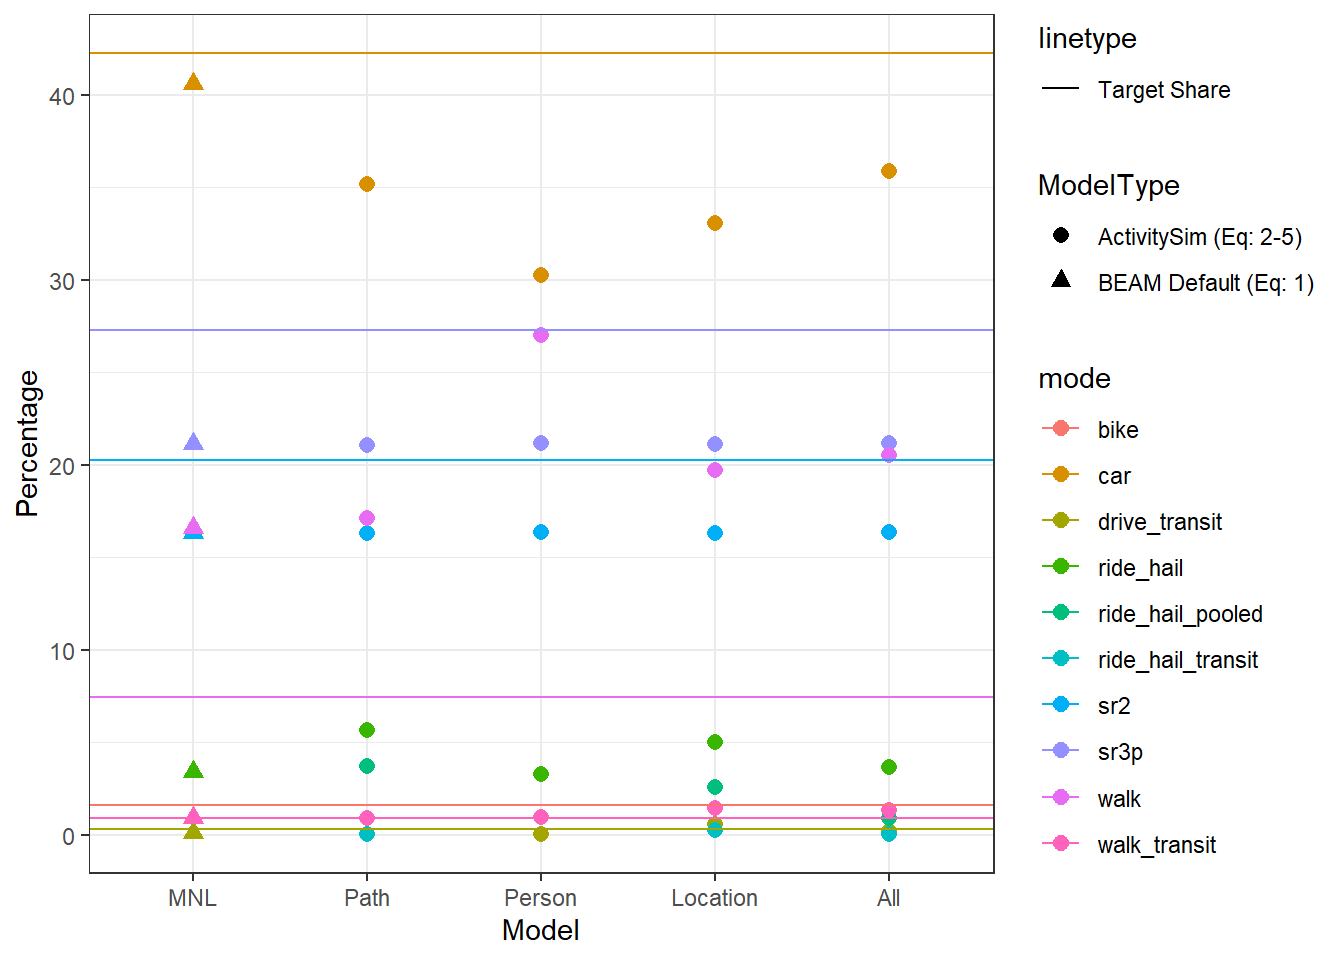
\includegraphics[width=0.8\linewidth]{mode_choice_calibration_files/figure-latex/fig1-1} 

}

\caption{The total modal split of each scenario compared with real world data.}\label{fig:fig1}
\end{figure}

Figure \ref{fig:fig2} displays how modal share is affected by vehicle ownership. Again, we were incorrect in our hypothesis that the ActivitySim All model \eqref{eq:label5} would align closest to the target shares. The Person model \eqref{eq:label3} best predicted the auto deficient values, the Path model \eqref{eq:label2} best predicted the auto sufficient values, and the BEAM Default MNL model \eqref{eq:label1} best predicted the no auto values. In general though, none of the models gave an accurate representation of this modal share.

\begin{figure}

{\centering 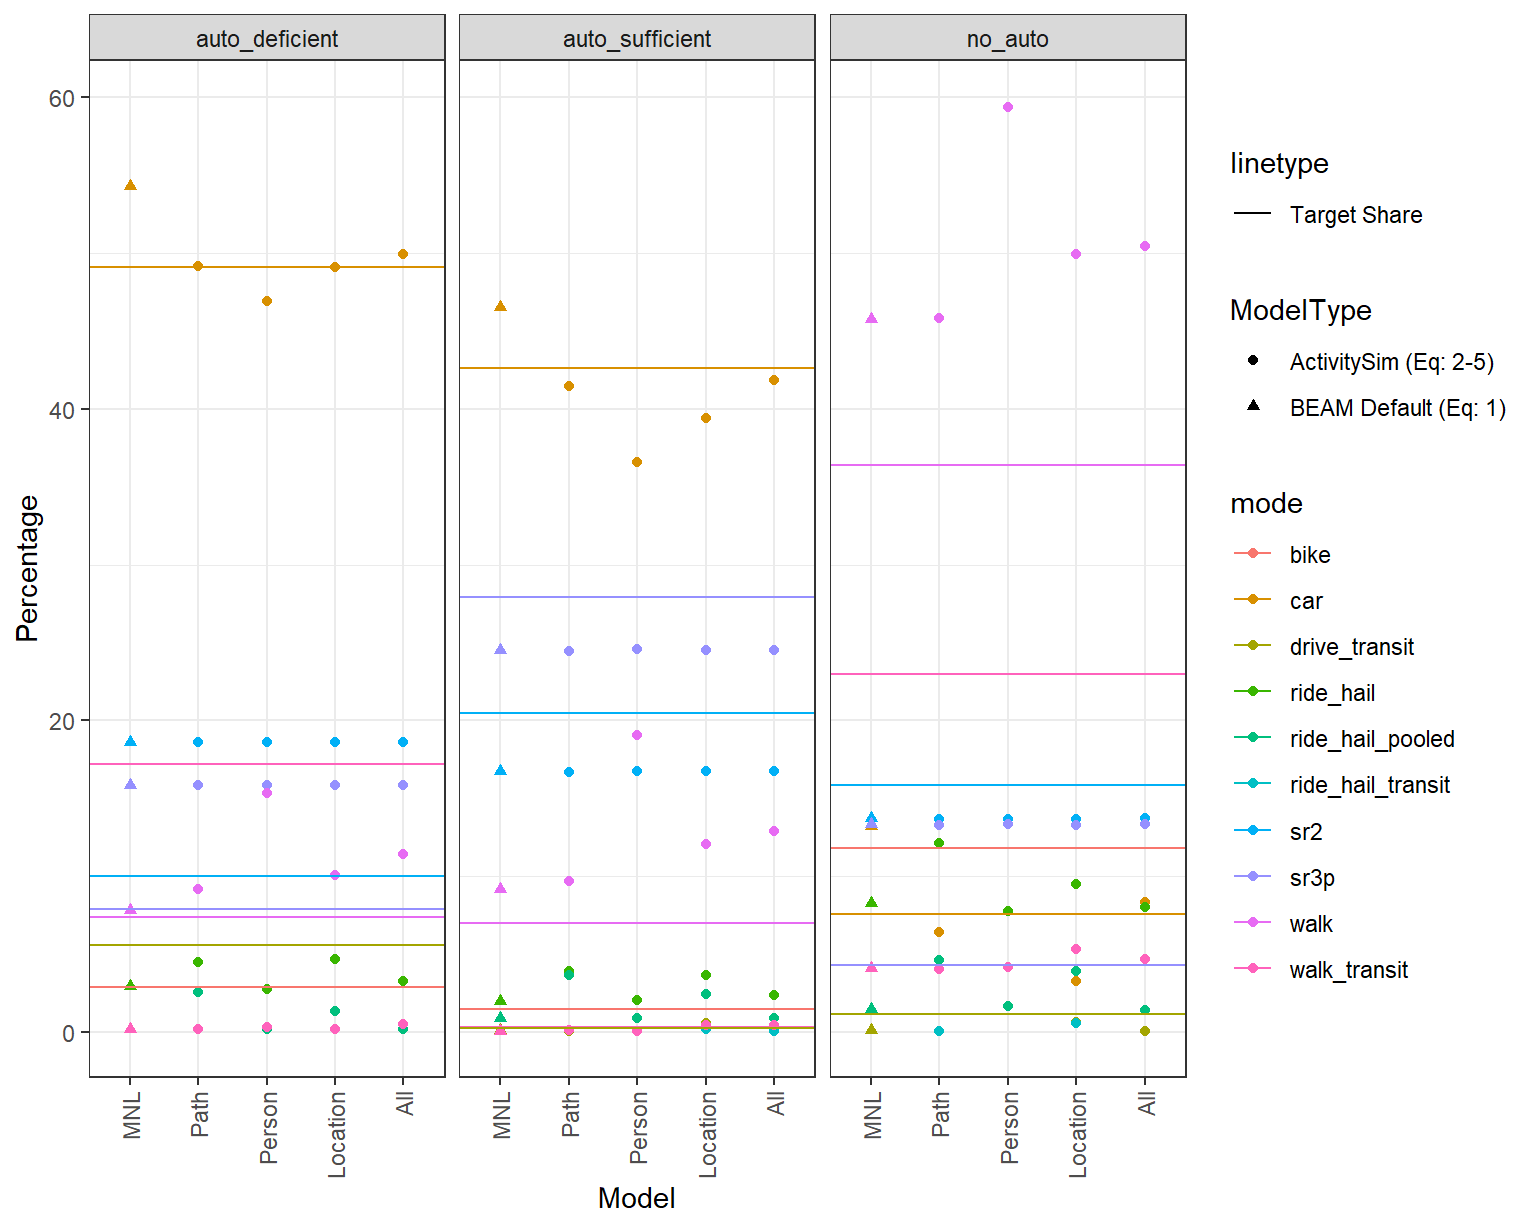
\includegraphics[width=0.8\linewidth]{mode_choice_calibration_files/figure-latex/fig2-1} 

}

\caption{The modal split by vehicle ownership of each scenario compared with real world data.}\label{fig:fig2}
\end{figure}

Figure \ref{fig:fig1} and Figure \ref{fig:fig2} also show that different variable types in the utility equation yield different mode choice results. The Path \eqref{eq:label2}, Person \eqref{eq:label3}, and Location \eqref{eq:label4} attributes all affected the mode choice in different ways.

Figure \ref{fig:fig3} displays how mode choice for each scenario is affected by tour purpose. School, university, and work purpose trips varied the most among different scenarios.

\begin{figure}

{\centering 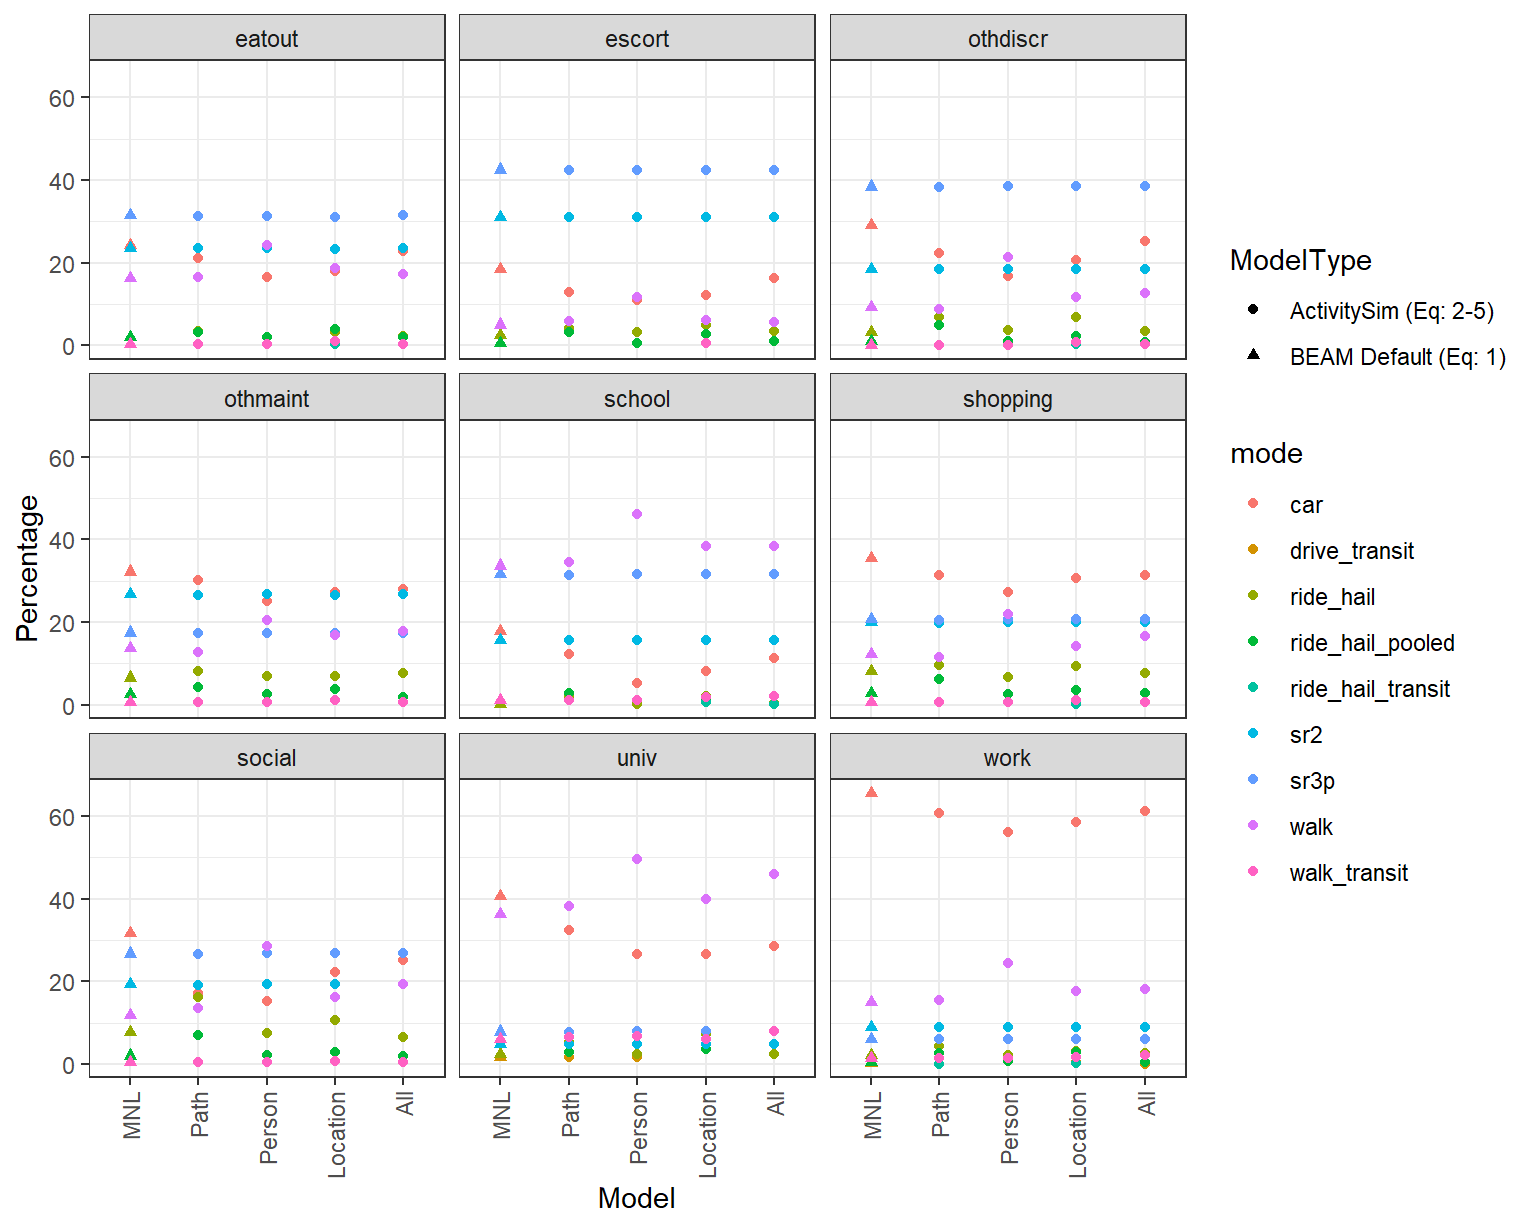
\includegraphics[width=0.8\linewidth]{mode_choice_calibration_files/figure-latex/fig3-1} 

}

\caption{The modal split by tour purpose of each scenario.}\label{fig:fig3}
\end{figure}

Overall, a microsimulation tool with a mode choice structure that mimics that of its parenting activity-based model does not seem to simulate mode choices accurately. However, we suggest that analysts attempt to rerun the scenarios that we have presented. Unfortunately, we did not calibrate the alternative specific constants for the ActivitySim scenarios. Rerunning the ActivitySim scenarios, but with calibrated constants, could yield more enticing results.

\hypertarget{acknowledgements}{%
\section{Acknowledgements}\label{acknowledgements}}

We are grateful to the Lawrence Berkeley National Laboratory for providing the BEAM software used to run each of our scenarios. We are also grateful to Wasatch Front Regional Council (WFRC) and the Metropolitan Planning Committee (MTC) for providing the data used to build our scenarios.

\hypertarget{references}{%
\section{References}\label{references}}

\bibliography{book.bib}


\end{document}

